\documentclass[11pt,preprint]{elsarticle}

\usepackage{lmodern}
%%%% My spacing
\usepackage{setspace}
\setstretch{1.2}
\DeclareMathSizes{12}{14}{10}{10}

% Wrap around which gives all figures included the [H] command, or places it "here". This can be tedious to code in Rmarkdown.
\usepackage{float}
\let\origfigure\figure
\let\endorigfigure\endfigure
\renewenvironment{figure}[1][2] {
    \expandafter\origfigure\expandafter[H]
} {
    \endorigfigure
}

\let\origtable\table
\let\endorigtable\endtable
\renewenvironment{table}[1][2] {
    \expandafter\origtable\expandafter[H]
} {
    \endorigtable
}


\usepackage{ifxetex,ifluatex}
\usepackage{fixltx2e} % provides \textsubscript
\ifnum 0\ifxetex 1\fi\ifluatex 1\fi=0 % if pdftex
  \usepackage[T1]{fontenc}
  \usepackage[utf8]{inputenc}
\else % if luatex or xelatex
  \ifxetex
    \usepackage{mathspec}
    \usepackage{xltxtra,xunicode}
  \else
    \usepackage{fontspec}
  \fi
  \defaultfontfeatures{Mapping=tex-text,Scale=MatchLowercase}
  \newcommand{\euro}{€}
\fi

\usepackage{amssymb, amsmath, amsthm, amsfonts}

\def\bibsection{\section*{References}} %%% Make "References" appear before bibliography


\usepackage[numbers]{natbib}

\usepackage{longtable}
\usepackage[margin=2.3cm,bottom=2cm,top=2.5cm, includefoot]{geometry}
\usepackage{fancyhdr}
\usepackage[bottom, hang, flushmargin]{footmisc}
\usepackage{graphicx}
\numberwithin{equation}{section}
\numberwithin{figure}{section}
\numberwithin{table}{section}
\setlength{\parindent}{0cm}
\setlength{\parskip}{1.3ex plus 0.5ex minus 0.3ex}
\usepackage{textcomp}
\renewcommand{\headrulewidth}{0.2pt}
\renewcommand{\footrulewidth}{0.3pt}

\usepackage{array}
\newcolumntype{x}[1]{>{\centering\arraybackslash\hspace{0pt}}p{#1}}

%%%%  Remove the "preprint submitted to" part. Don't worry about this either, it just looks better without it:
\makeatletter
\def\ps@pprintTitle{%
  \let\@oddhead\@empty
  \let\@evenhead\@empty
  \let\@oddfoot\@empty
  \let\@evenfoot\@oddfoot
}
\makeatother

 \def\tightlist{} % This allows for subbullets!

\usepackage{hyperref}
\hypersetup{breaklinks=true,
            bookmarks=true,
            colorlinks=true,
            citecolor=blue,
            urlcolor=blue,
            linkcolor=blue,
            pdfborder={0 0 0}}


% The following packages allow huxtable to work:
\usepackage{siunitx}
\usepackage{multirow}
\usepackage{hhline}
\usepackage{calc}
\usepackage{tabularx}
\usepackage{booktabs}
\usepackage{caption}


\newenvironment{columns}[1][]{}{}

\newenvironment{column}[1]{\begin{minipage}{#1}\ignorespaces}{%
\end{minipage}
\ifhmode\unskip\fi
\aftergroup\useignorespacesandallpars}

\def\useignorespacesandallpars#1\ignorespaces\fi{%
#1\fi\ignorespacesandallpars}

\makeatletter
\def\ignorespacesandallpars{%
  \@ifnextchar\par
    {\expandafter\ignorespacesandallpars\@gobble}%
    {}%
}
\makeatother


% definitions for citeproc citations
\NewDocumentCommand\citeproctext{}{}
\NewDocumentCommand\citeproc{mm}{%
\href{\#cite.\detokenize{#1}}{#2}\nocite{#1}}

\makeatletter
% allow citations to break across lines
\let\@cite@ofmt\@firstofone
% avoid brackets around text for \cite:
\def\@biblabel#1{}
\def\@cite#1#2{{#1\if@tempswa , #2\fi}}
\makeatother
\newlength{\cslhangindent}
\setlength{\cslhangindent}{1.5em}
\newlength{\csllabelwidth}
\setlength{\csllabelwidth}{3em}
\newenvironment{CSLReferences}[2] % #1 hanging-indent, #2 entry-spacing
{\begin{list}{}{%
	\setlength{\itemindent}{0pt}
	\setlength{\leftmargin}{0pt}
	\setlength{\parsep}{0pt}
	% turn on hanging indent if param 1 is 1
	\ifodd #1
	\setlength{\leftmargin}{\cslhangindent}
	\setlength{\itemindent}{-1\cslhangindent}
	\fi
	% set entry spacing
	\setlength{\itemsep}{#2\baselineskip}}}
{\end{list}}

\usepackage{calc}
\newcommand{\CSLBlock}[1]{\hfill\break\parbox[t]{\linewidth}{\strut\ignorespaces#1\strut}}
\newcommand{\CSLLeftMargin}[1]{\parbox[t]{\csllabelwidth}{\strut#1\strut}}
\newcommand{\CSLRightInline}[1]{\parbox[t]{\linewidth - \csllabelwidth}{\strut#1\strut}}
\newcommand{\CSLIndent}[1]{\hspace{\cslhangindent}#1}


\urlstyle{same}  % don't use monospace font for urls
\setlength{\parindent}{0pt}
\setlength{\parskip}{6pt plus 2pt minus 1pt}
\setlength{\emergencystretch}{3em}  % prevent overfull lines
\setcounter{secnumdepth}{5}

%%% Use protect on footnotes to avoid problems with footnotes in titles
\let\rmarkdownfootnote\footnote%
\def\footnote{\protect\rmarkdownfootnote}
\IfFileExists{upquote.sty}{\usepackage{upquote}}{}

%%% Include extra packages specified by user

%%% Hard setting column skips for reports - this ensures greater consistency and control over the length settings in the document.
%% page layout
%% paragraphs
\setlength{\baselineskip}{12pt plus 0pt minus 0pt}
\setlength{\parskip}{12pt plus 0pt minus 0pt}
\setlength{\parindent}{0pt plus 0pt minus 0pt}
%% floats
\setlength{\floatsep}{12pt plus 0 pt minus 0pt}
\setlength{\textfloatsep}{20pt plus 0pt minus 0pt}
\setlength{\intextsep}{14pt plus 0pt minus 0pt}
\setlength{\dbltextfloatsep}{20pt plus 0pt minus 0pt}
\setlength{\dblfloatsep}{14pt plus 0pt minus 0pt}
%% maths
\setlength{\abovedisplayskip}{12pt plus 0pt minus 0pt}
\setlength{\belowdisplayskip}{12pt plus 0pt minus 0pt}
%% lists
\setlength{\topsep}{10pt plus 0pt minus 0pt}
\setlength{\partopsep}{3pt plus 0pt minus 0pt}
\setlength{\itemsep}{5pt plus 0pt minus 0pt}
\setlength{\labelsep}{8mm plus 0mm minus 0mm}
\setlength{\parsep}{\the\parskip}
\setlength{\listparindent}{\the\parindent}
%% verbatim
\setlength{\fboxsep}{5pt plus 0pt minus 0pt}



\begin{document}



\begin{frontmatter}  %

\title{Coldplay and Metallica}

% Set to FALSE if wanting to remove title (for submission)




\author[Add1]{Matthew Thompson}
\ead{22892435@sun.ac.za}





\address[Add1]{Department of Economics, Stellenbosch University}



\vspace{1cm}





\vspace{0.5cm}

\end{frontmatter}

\setcounter{footnote}{0}



%________________________
% Header and Footers
%%%%%%%%%%%%%%%%%%%%%%%%%%%%%%%%%
\pagestyle{fancy}
\chead{}
\rhead{}
\lfoot{}
\rfoot{\footnotesize Page \thepage}
\lhead{}
%\rfoot{\footnotesize Page \thepage } % "e.g. Page 2"
\cfoot{}

%\setlength\headheight{30pt}
%%%%%%%%%%%%%%%%%%%%%%%%%%%%%%%%%
%________________________

\headsep 35pt % So that header does not go over title




\section{\texorpdfstring{Introduction
\label{Introduction}}{Introduction }}\label{introduction}

\section{Clean and remove live songs}\label{clean-and-remove-live-songs}

First we want to make sure song durations is measured the same for both
bands. Need to convert duration column in Metallica's dataset (currently
in milliseconds) into seconds.

Next want to get release dates as years only and make sure column names
are the same in both dataframes to make for easier coding later.

Now want to filter out all the live songs.

\section{Song length over time}\label{song-length-over-time}

The analysis starts by simply examining how the length of song released
by each band varied over time.

Below we plot the average song duration for both Metallica and Coldplay
over time.

\begin{figure}[H]

{\centering 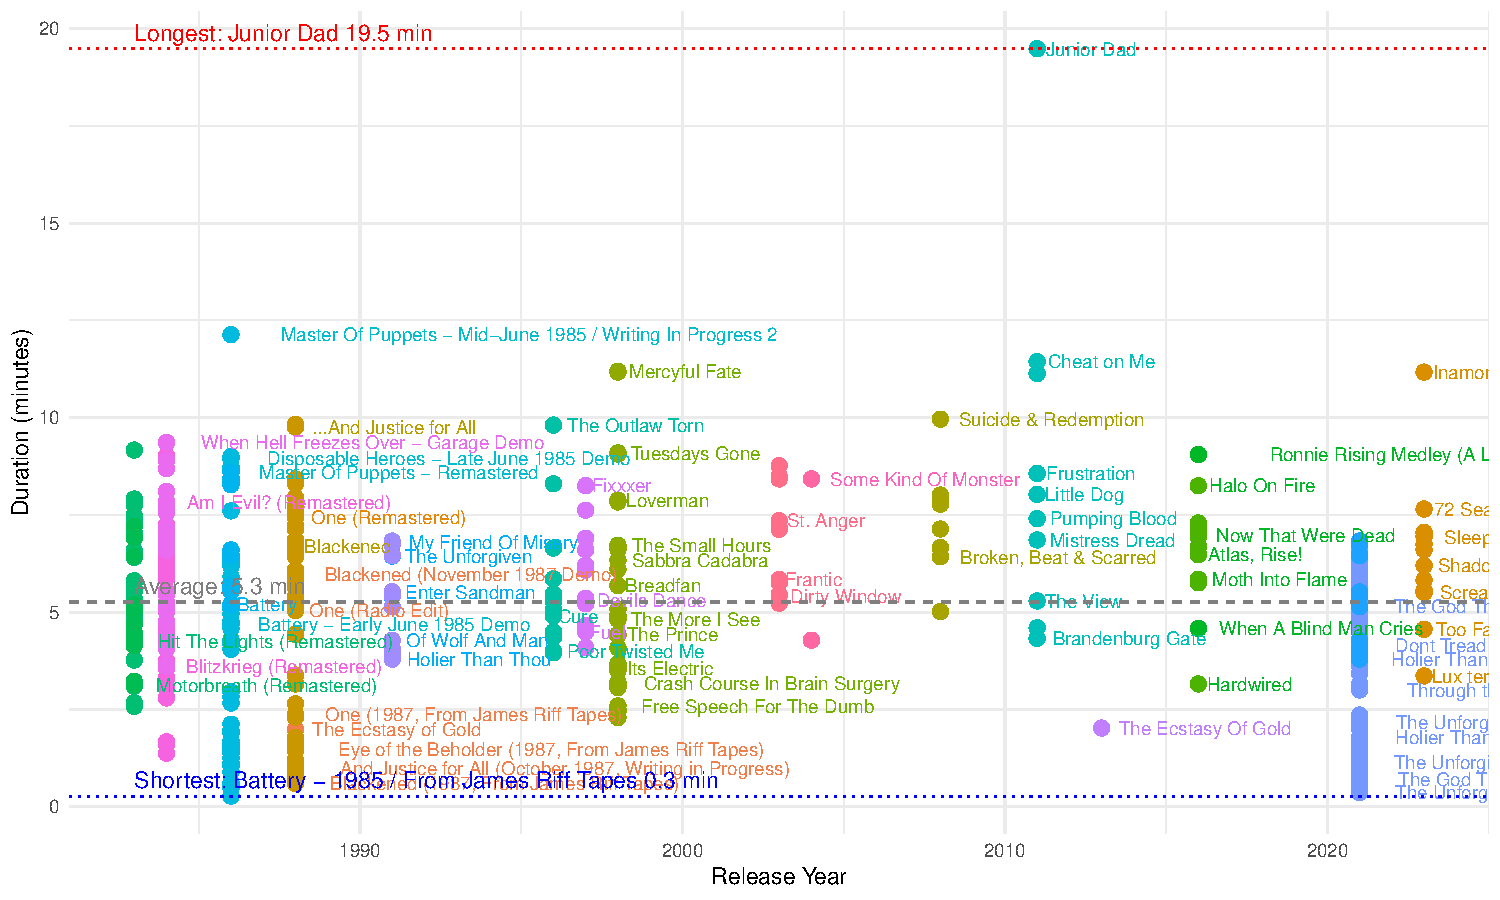
\includegraphics[width=0.8\linewidth]{./output/fig1} 

}

\caption{Plot showing Metallica song durations over time \label{Fig1}}\label{fig:unnamed-chunk-4}
\end{figure}

Now want to perform the same for Coldplay

\begin{figure}[H]

{\centering 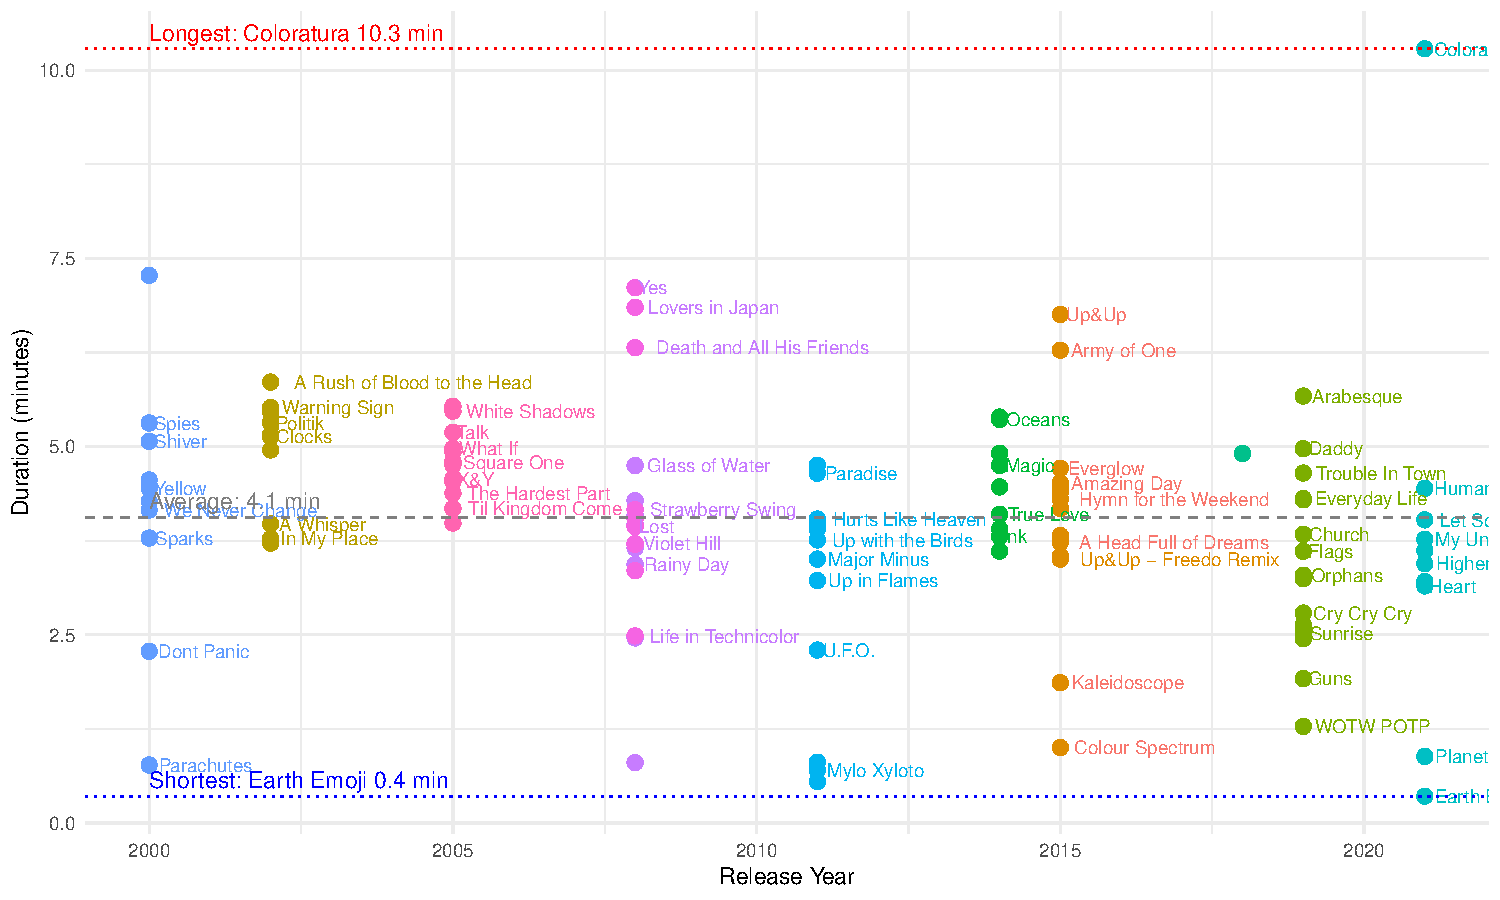
\includegraphics[width=0.8\linewidth]{./output/fig2} 

}

\caption{Plot showing Coldplay song durations over time \label{Fig2}}\label{fig:unnamed-chunk-6}
\end{figure}

The above graphs show the following interesting summary statistics:

\begin{itemize}
\tightlist
\item
  Metallica had a longer average song duration.
\item
  Metallica's longest song is almost double that of Coldplay's.
\item
  Metallica also has the shortest length of song between the two bands.
\end{itemize}

\section{Danceability comparison (Studio vs Live
comparison)}\label{danceability-comparison-studio-vs-live-comparison}

One of the hallmarks of music is being able to dance to a good set. This
section compares the difference in the danceability between Coldplay and
Metallica throughout each of their albums. It then also compares this
only for their live performances, to see if there is a big difference
which exists between their studio-recorded, and demo performances etc.,
and their live shows.

\begin{figure}[H]

{\centering 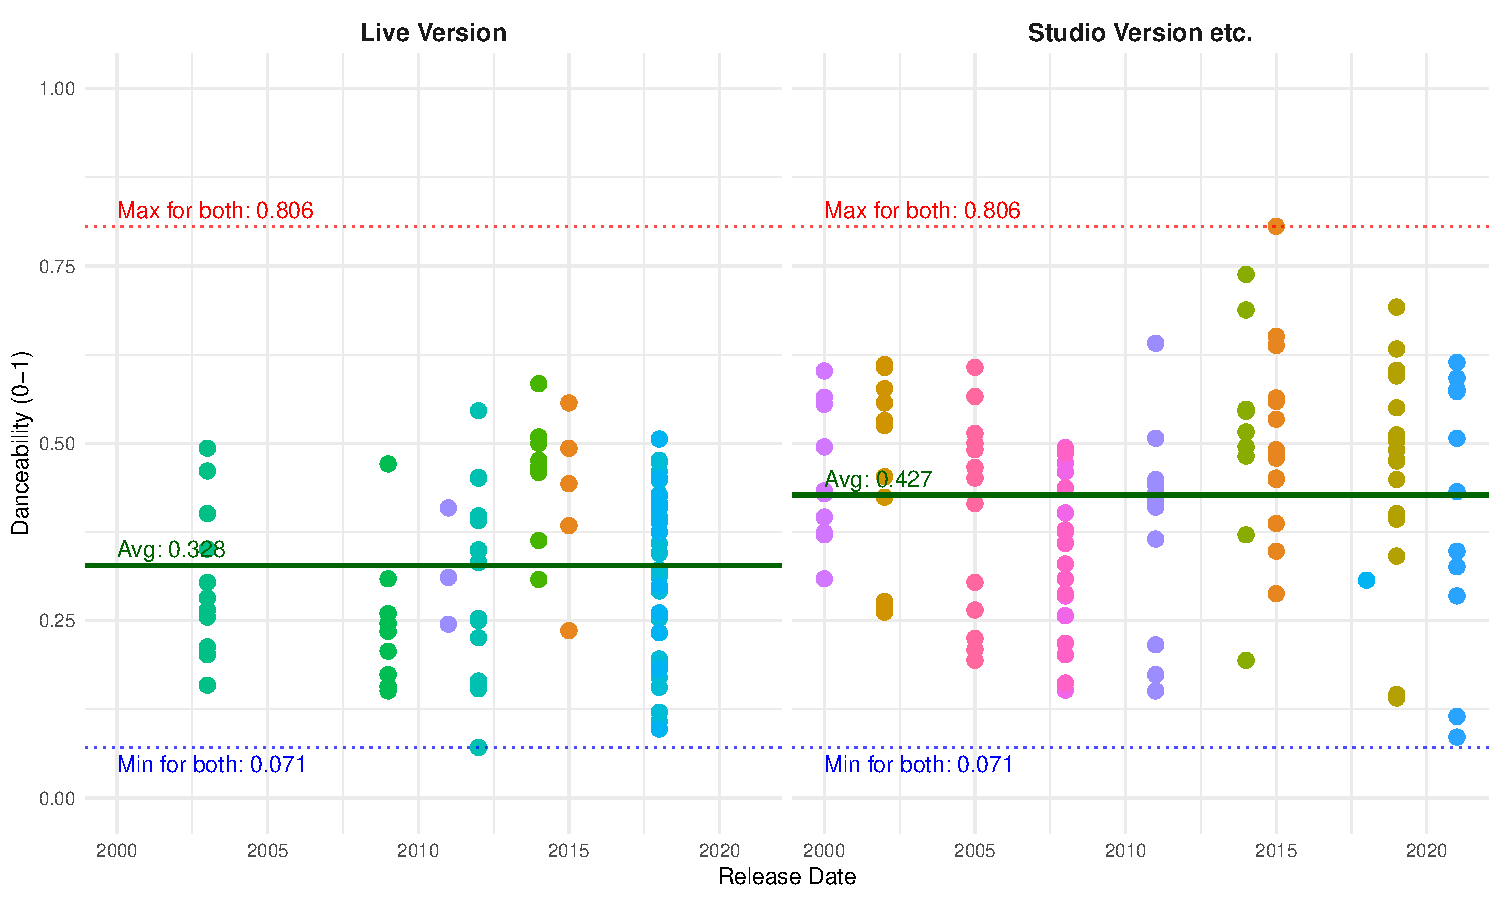
\includegraphics[width=0.8\linewidth]{./output/fig3} 

}

\caption{Plot showing Coldplay danceability difference between different recording types \label{Fig3}}\label{fig:unnamed-chunk-8}
\end{figure}

When looking at Coldplay in Figure \ref{Fig3}, we see that their studio
and other versions (everything but Live recordings) displays a higher
danceability than their live shows, implying that the latter tends to
have a more down-beat atmosphere.

\begin{figure}[H]

{\centering 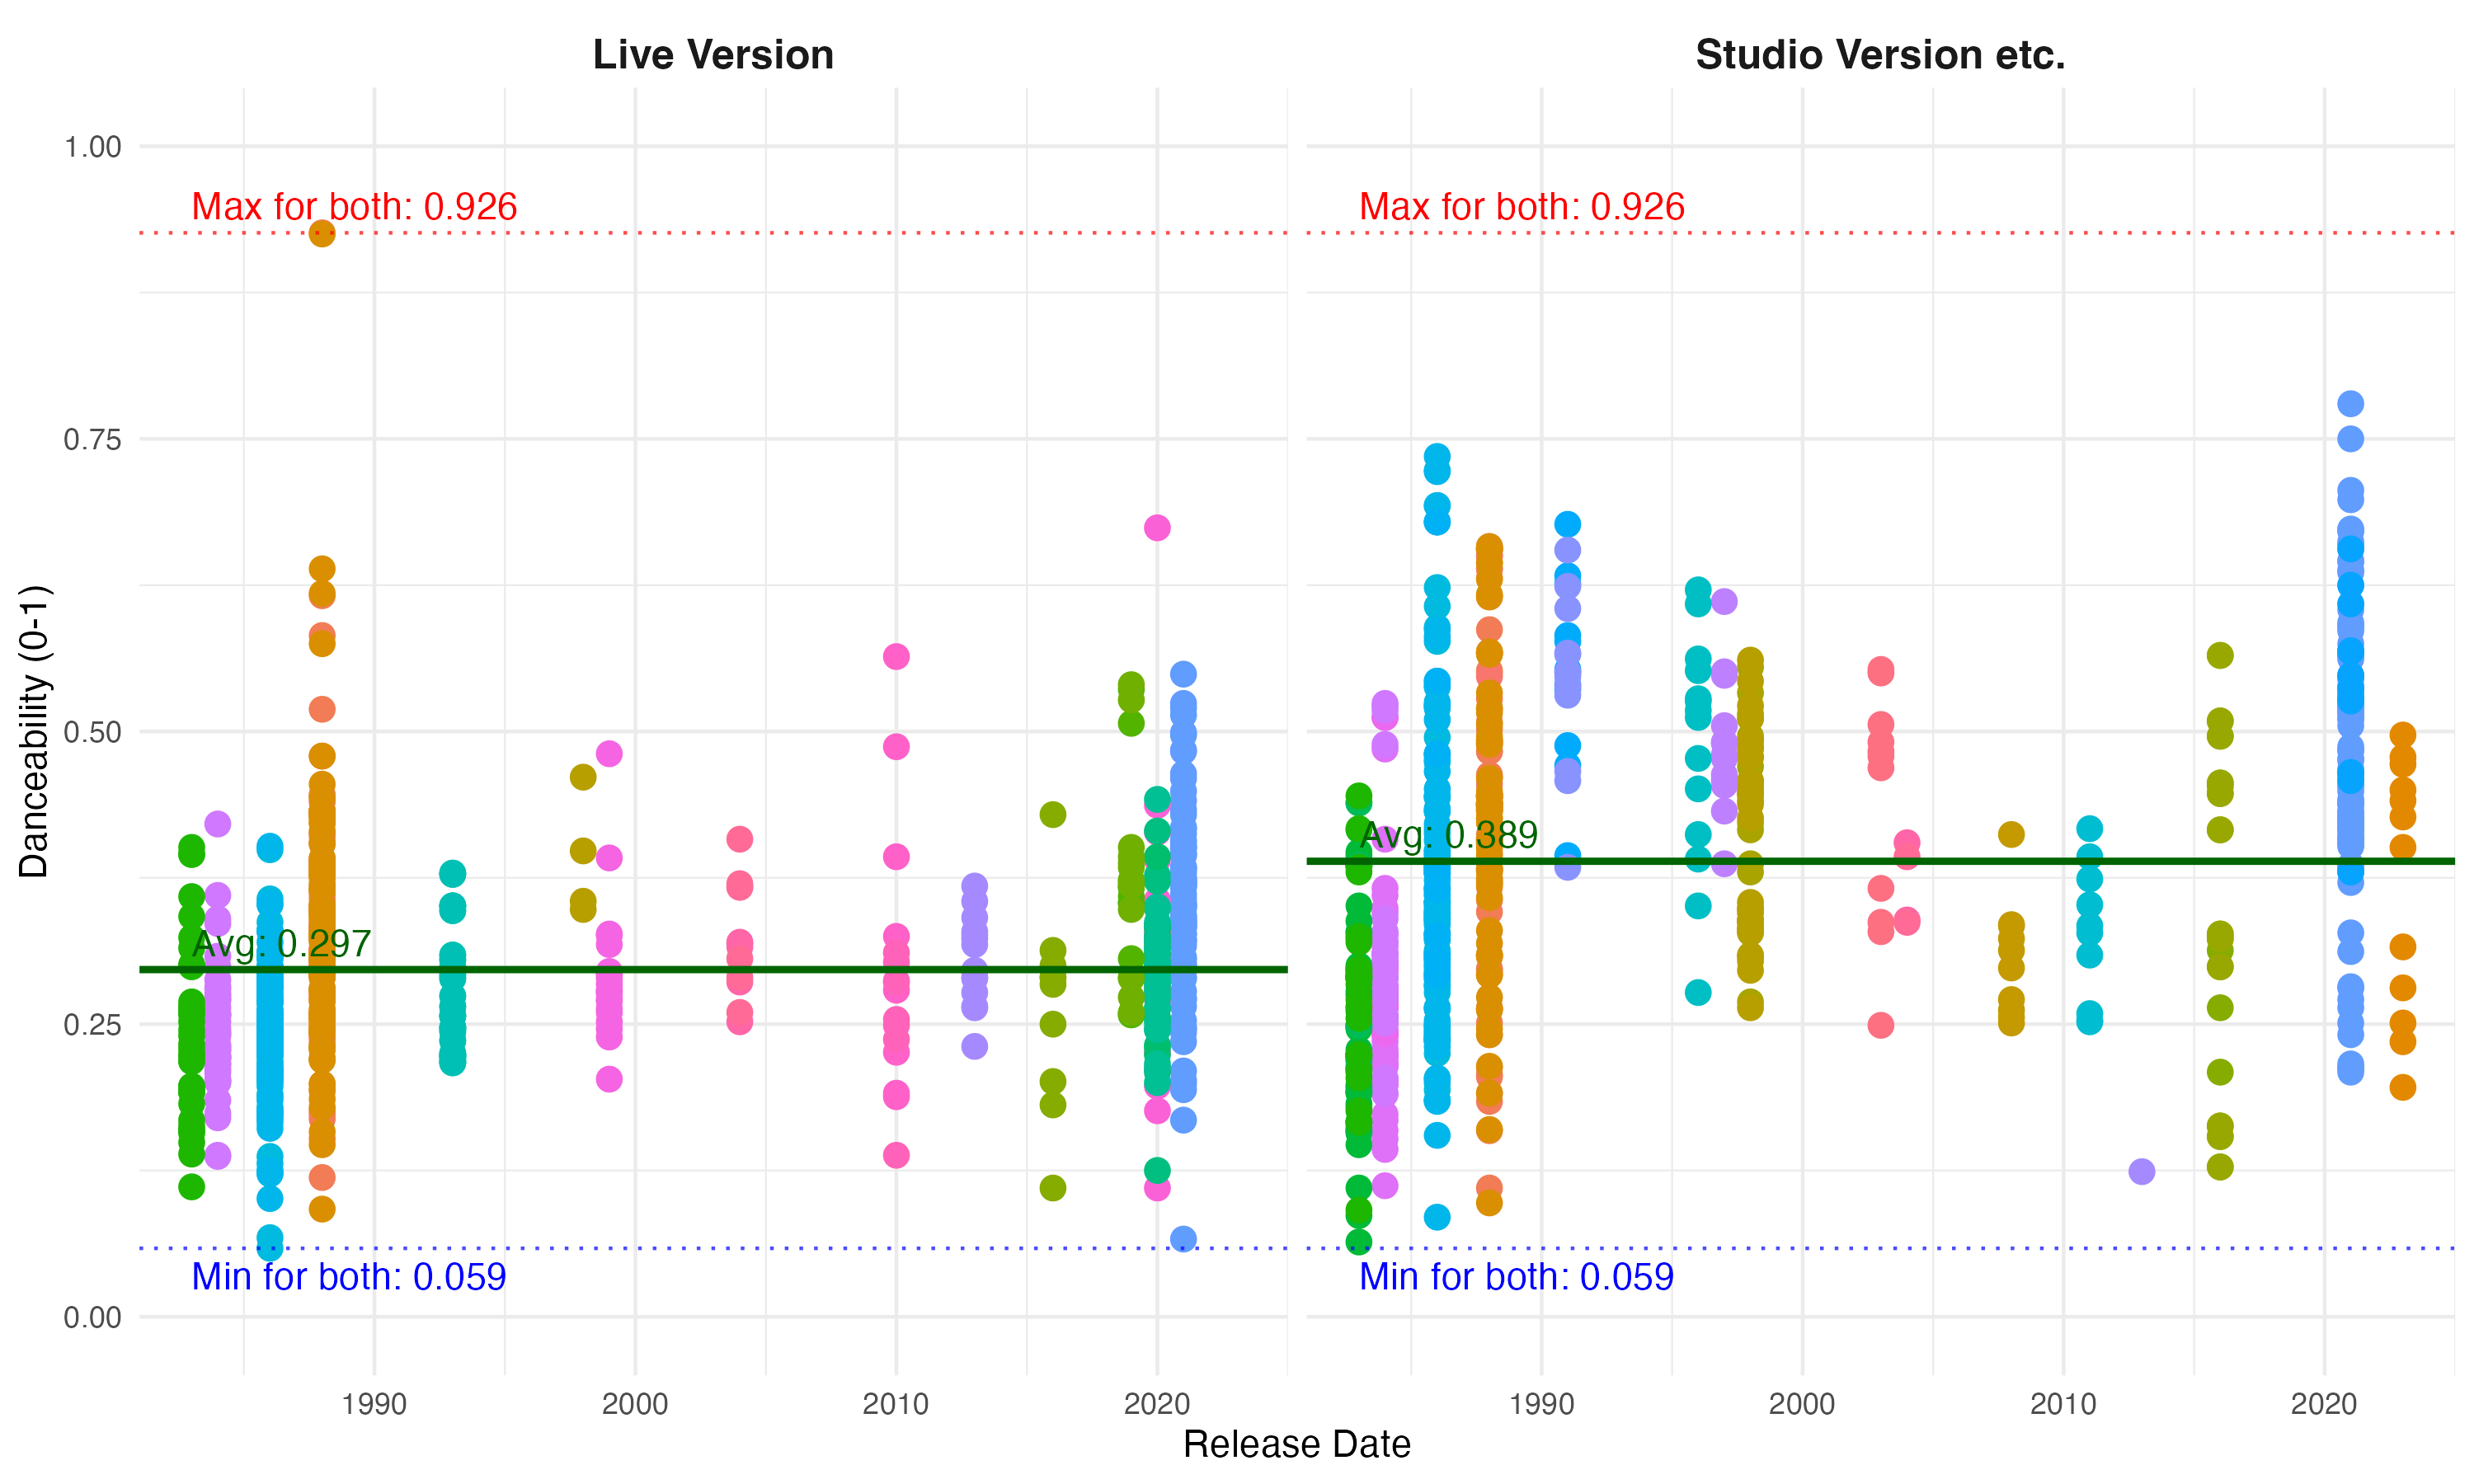
\includegraphics[width=0.8\linewidth]{./output/fig4} 

}

\caption{Plot showing Metallica danceability difference between different recording types  \label{Fig4}}\label{fig:unnamed-chunk-10}
\end{figure}

We see that in the case of Metallica, live shows are similarly less
suited for dancing than their studio recordings.\\
This contradicts literature which states that live performances often
bring out more energy and emotion, seen through better danceability
scores (\citeproc{ref-swarbrick2019}{Swarbrick, Bosnyak, Livingstone,
Bansal, Marsh-Rollo, Woolhouse \& Trainor, 2019}).

\newpage

\section*{References}\label{references}
\addcontentsline{toc}{section}{References}

\phantomsection\label{refs}
\begin{CSLReferences}{1}{1}
\bibitem[\citeproctext]{ref-swarbrick2019}
Swarbrick, D., Bosnyak, D., Livingstone, S.R., Bansal, J., Marsh-Rollo,
S., Woolhouse, M.H. \& Trainor, L.J. 2019. How live music moves us: Head
movement differences in audiences to live versus recorded music.
\emph{Frontiers in psychology}. 9:2682.

\end{CSLReferences}

\bibliography{Tex/ref}





\end{document}
